\chapter{Tests on Categorical Data }

In a data sample the number of data falling into a particular group is called the Frequency, so the analysis of categorical data is the analysis of frequencies. When two or more groups are compared the data are often shown in the form of a \emph{frequency table}, sometimes also called \emph{contingency table}. For example, Table \ref{table:frequency} gives the number of right/left-handed subjects, \emph{contingent} on the subject being male or female.

\begin{table}
  \centering
  \begin{tabular}{|c|l l l|}
  \hline
  & \emph{Right Handed} & \emph{Left Handed} & \emph{Total} \\
  \hline
  \emph{Males} & 43 & 9 & 52 \\
  \emph{Females} & 44 & 4 & 48 \\
  \emph{Total} & 87 & 13 & 100 \\
  \hline
  \end{tabular}

  \caption{Example of a frequency table}\label{table:frequency}
\end{table}

If you have only one sample group of data, the analysis options are somewhat limited. In contrast, a number of statistical tests exist for the analysis of frequency tables.

\begin{description}
  \item[Chi-square test] This is the most common type. It is a hypothesis test, which checks if the entries in the individual cells all come from the same distribution. In other words, it checks the null hypothesis $H_0$ that the results are independent of the row or column in which they appear. The alternative hypothesis $H_a$ does not specify the type of association, so close attention to the data is required to interpret the information provided by the test.
  \item[Fisher's Exact Test] While the chi-square test is approximate, the \emph{Fisher's Exact Test} is an exact test. As it is computationally much more expensive and intricate than the chi-square test, it was originally used only for small sample numbers. However, in general it is now the more advisable test to use.
  \item[McNemar's Test]  This is a \emph{matched pair test }for 2x2 tables.
  \item[Cochran's Q Test] \index{general}{test!Cochran's Q} Cochran's Q test is an extension to the McNemar's test for related samples that provides a method for testing for differences between three or more \emph{matched/paired} sets of frequencies or proportions. For example, if you have exactly the same samples analyzed by 3 different laboratories, and you want to check if the results are statistically equivalent, you would use this test.
\end{description}


\section{One Proportion}

If you have one sample group of data, you can check if your sample is representative of the standard population. To do so, you have to know the proportion $p$ of the characteristic in the standard population. The occurrence of a characteristic in a group of $n$ people is described by the binomial distribution, with $mean = p*n$. The standard error of samples with this characteristic is given by

\begin{equation}\label{eq:oneProportion}
  se(p) = \sqrt{p(1-p)/n}
\end{equation}

and the corresponding 95\% confidence interval is
\begin{equation*}
  ci = mean \pm se * t_{n,0.95}
\end{equation*}

If your data lie outside this confidence interval, they are \emph{not} representative of the population.

\subsection{Explanation}

The innocent looking equation \ref{eq:oneProportion} is more involved than it seems at first:

If you have $n$ independent samples from a binomial distribution $B(k,p)$, the variance of their sample mean is

\begin{equation*}
    \operatorname{var} \left( {\frac{1}{n}\sum\limits_{i = 1}^n {{X_i}} } \right) = \frac{1}{{{n^2}}}\sum\limits_{i = 1}^n {\operatorname{var} ({X_i})}  = \frac{{n\,\operatorname{var} ({X_i})}}{{{n^2}}} = \frac{{\operatorname{var} ({X_i})}}{n} = \frac{{kpq}}{n}
\end{equation*}

where $q=1−p$ and $\bar{X}$ is the same mean. This follows since
\begin{enumerate}
  \item $var(cX)=c^2 var(X)$, for any random variable, $X$, and any constant $c$.
  \item the variance of a sum of independent random variables equals the sum of the variances.
\end{enumerate}

The standard error of $\bar{X}$ is the square root of the variance: $\sqrt {\frac{kpq}{n}}$. Therefore,

\begin{itemize}
  \item When $k=n$, we get $se = \sqrt {pq}$.
  \item When $k=1$, and the Binomial variables are just Bernoulli trials, the standard error is given by $se = \sqrt {\frac{pq}{n}}$.
\end{itemize}


\subsection{Example}

For example, let us look at incidence and mortality for breast cancer, and try to answer the following two questions: among the FH-students, how many occurrences of breast cancer should we expect per year? And how many of the female FH-students will probably die from breast cancer at the end of their life?

We know that:

\begin{itemize}
  \item the FH OOe has about 5'000 students, about half of which are female.
  \item breast cancer hits predominantly women.
  \item the \emph{incidence} of breast cancer in the age group 20-30 is about 10, where \emph{incidence}\index{general}{incidence} is typically defined as the new occurrences of a disease per year per 100'000 people.
  \item 3.8\% of all women die of cancer.
\end{itemize}

From these points of information, we can obtain the following parameters for our calculations

\begin{itemize}
  \item n = 2'500
  \item $p_{incidence} = 10 / 100'000$
  \item $p_{mortality} = 3.8/100$.
\end{itemize}

The 95\% confidence interval for the incidence is -0.7 - 1.2, and for the number of deaths 76 - 114. So we expect that every year most likely none or one of the FH-students will be diagnosed with breast cancer; but between 76 and 114 of the female students will eventually die from this disease.

\section{Frequency Tables} \index{general}{frequency tables}

If your data can be organized in a set of categories, and they are given as \emph{frequencies}, i.e. the total number of samples in each category (not as percentages), the tests described in this section are appropriate for your data analysis.

Many of these tests analyze the \emph{deviation from an expected value}. Since the chi-square distribution characterizes the variability of data (in other words, their deviation from a mean value), many of these tests refer to this distribution, and are accordingly termed \emph{chi-square tests}.

\begin{table}
  \centering
  \begin{tabular}{|c|l l l|}
  \hline
  & \emph{Right Handed} & \emph{Left Handed} & \emph{Total} \\
  \hline
  \emph{Males} & 45.2 & 6.8 & 52 \\
  \emph{Females} & 41.8 & 6.2 & 48 \\
  \emph{Total} & 87 & 13 & 100 \\
  \hline
  \end{tabular}

  \caption{Corresponding \emph{expected values} for Table \ref{table:frequency}\label{table:expectedValues}}
\end{table}


Assume that you have observed absolute frequencies $o_i$ and expected absolute frequencies $e_i$. Under the Null hypothesis all your data come from the same population, and the test statistic

\begin{equation}\label{eq:chi2}
  V = \sum_i \frac{(o_i-e_i)^2}{e_i} \approx \chi^2_f
\end{equation}.

follows a chi square distribution with $f$ degrees of freedom. $i$ might denote a simple index running from $1,...,I$ or a multiindex $(i_1,...,i_p)$ running from $(1,...,1)$ to $(I_1,...,I_p)$.

\subsection{One-way Chi-square Test}\index{general}{test!chi square, one way}

For example, assume that you go hiking with your friends. Every evening, you draw lots who has to do the washing up.
But at the end of the trip, you seem to have done most of the work:

\begin{table}[h]
    \centering
    \begin{tabular}{c|c|c|c|c|c}
      You & Peter & Hans & Paul & Mary & Joe \\
      \hline
      10 & 6 & 5 & 4 & 5 & 3 \\
    \end{tabular}
\end{table}

You expect that there has been some foul play, and calculate how likely it is that this distribution came up by chance. The

\begin{equation}
  expectedFrequency = \frac{n_{total}}{n_{people}}
\end{equation}

is 5.5. The likelihood that this distribution came up by chance is

\begin{lstlisting}[language=Python]
    V, p = stats.chisquare(data)
    print(p)
    >>> 0.373130385949
\end{lstlisting}

In other words, you doing a lot of the washing up really could have been by chance!

\subsection{Chi-square Contingency Test} \index{general}{test!chi square}

If you can arrange your data in rows and columns, you can check if the numbers in the individual columns are contingent on the row value. For this reason, this test is sometimes called Contingency Test.

The chi-square contingency test is based on a test statistic that measures the divergence of the observed data from the values that would be expected under the null hypothesis of no association (e.g. Table \ref{table:expectedValues}). When $n$ is the total number of observations included in the table, the expected value for each cell in a two-way table is

\begin{equation}
  expectedFrequency = \frac{RowTotal * ColumnTotal}{n}
\end{equation}


\subsubsection{Assumptions}
The test statistic $V$ is approximately $\chi^2$ distributed, if

\begin{itemize}
  \item for all absolute expected frequencies $e_i$ holds $e_i \geq 1$ and
  \item for at least 80\% of the absolute expected frequencies $e_i$ holds $e_i \geq 5$.
\end{itemize}

For small sample numbers, corrections should be made for some bias that is caused by the use of the continuous chi-squared distribution, while the frequencies are by definition integers. This correction is referred to as \emph{Yates correction}.

\subsubsection{Degrees of Freedom}
The degrees of freedom (DOF) can be computed by the numbers of absolute observed frequencies which can be chosen freely. For example, only one cell of a 2x2 table with the sums at the side and bottom needs to be filled, and the others can be found by subtraction. In general, an $r \times c$ table has $df=(r-1)\times(c-1)$ degrees of freedom.
 We know that the sum of absolute expected frequencies is

\begin{equation}
  \sum_i o_i = n
\end{equation}

We might have to subtract from the number of degrees of freedom the number of parameters we need to estimate from the sample, since this implies further relationships between the observed frequencies.

\subsubsection{Example 1}

The \emph{Python} command \emph{stats.chi2\_contingency} returns the following list: ($\chi^2$-value, p-value, degrees-of-freedom, expected values).

\begin{lstlisting}[language=Python]
     data = np.array([[43,9],
                      [44,4]])
    V, p, dof, expected = stats.chi2_contingency(data)
    print(p)
    >>> 0.300384770391
\end{lstlisting}

For the example data in Table \ref{table:frequency}, the results are ($\chi^2=1.1, p=0.3, df=1$). In other words, there is no indication that there is a difference in left-handed people vs right-handed people between males and females.

\textbf{Note:} These values assume the default setting, which uses the \emph{Yates correction}. Without this correction, i.e. using Eq. \ref{eq:chi2}, the results are $\chi^2=1.8, p=0.18$.

\subsubsection{Example 2}

The Chi-square test can be used to generate a "quick and dirty" test of normality, e.g.

$H_0:$ The random variable $X$ is symmetrically distributed versus

$H_1:$ the random variable $X$ is not symmetrically distributed.

We know that in case of a symmetrical distribution the arithmetic mean $\bar{x}$ and median should be nearly the same. So a simple way to test this hypothesis would be to count how many observations  are less than the mean ($n_-$)and how many observations are larger than the arithmetic mean ($n_+$). If mean and median are the same than 50\% of the observation should smaller than the mean and 50\% should be larger than the mean. It holds

\begin{equation}
  V = \frac{(n_- - n/2)^2}{n/2} + \frac{(n_+ - n/2)^2}{n/2} \approx \chi^2_1
\end{equation}.


\subsubsection{Comments}

%[xxx Here I don't understand the reviewer's comment xxx]

The Chi-square test is a pure hypothesis test. It tells you if your observed frequency can be due to a random sample selection from a single population. A number of different expressions have been used for chi-square tests, which are due to the original derivation of the formulas (from the time before computers were pervasive). Expression such as \emph{2x2 tables}, \emph{r-c tables}, or \emph{Chi-square test of contingency} all refer to frequency tables and are typically analyzed with chi-square tests.


\subsection{Fisher's Exact Test} \index{general}{test!Fisher's exact}

\begin{table}
  \centering
  \begin{tabular}{|c|l l| l|}
  \hline
  &  & B &  \\
  & 1 & 0 & \emph{Totals} \\
  \hline
  A 1 & a & b & a+b \\
    0 & c & d & c+d \\
  \hline
  \emph{Totals} & a+c & b+d & N=a+b+c+d \\
  \hline
  \end{tabular}

  \caption{General Structure of 2x2 Frequency Tables}\label{table:frequencyGeneral}
\end{table}


If the requirement that 80\% of cells should have expected values of at least 5 is not fulfilled, \emph{Fisher's exact test} should be used. This test is based on the observed row and column totals. The method consists of evaluating the probability associated with all possible 2x2 tables which have the same row and column totals as the observed data, making the assumption that the null hypothesis (i.e. that the row and column variables are unrelated) is true.  In most cases, Fisher's exact test is preferable to the chi-square test. But until the advent of powerful computers, it was not practical. You should use it up to approximately 10-15 cells in the frequency tables. It is called "exact" because the significance of the deviation from a null hypothesis can be calculated exactly, rather than relying on an approximation that becomes exact in the limit as the sample size grows to infinity, as with many statistical tests.

% [xxx The reviewer marked the section "rather than relying on an approximation" - but I don't understand why xxx]

In using the test, you have to decide if you want to use a one-tailed test or a two-tailed test. The former one looks for the probability to find a distribution as extreme as or more extreme than the observed one. The latter one (which is the default in python) also considers tables as extreme in the opposite direction.

\textbf{Note:} The python command \lstinline{stats.fisher_exact} returns by default the p-value for \emph{finding a value as extreme or more extreme than the observed one}. According to Altman (\cite{altman99}), this is a reasonable approach, although not all statisticians agree on that point.

\subsubsection{Example: "A Lady Tasting Tea"}

\footnote{Adapted from Stat Labs: Mathematical statistics through applications by D. Nolan and T. Speed, Springer-Verlag, New York, 2000}R. A. Fisher was one of the founding fathers of modern statistics. One of his early, and perhaps the most famous, experiments was to test an English lady's claim that she could tell whether milk was poured before tea or not. Here is an account of the seemingly trivial event that had the most profound impact on the history of modern statistics, and hence, arguably, modern quantitative science \cite{Box1978}.

\begin{figure}
  \centering
  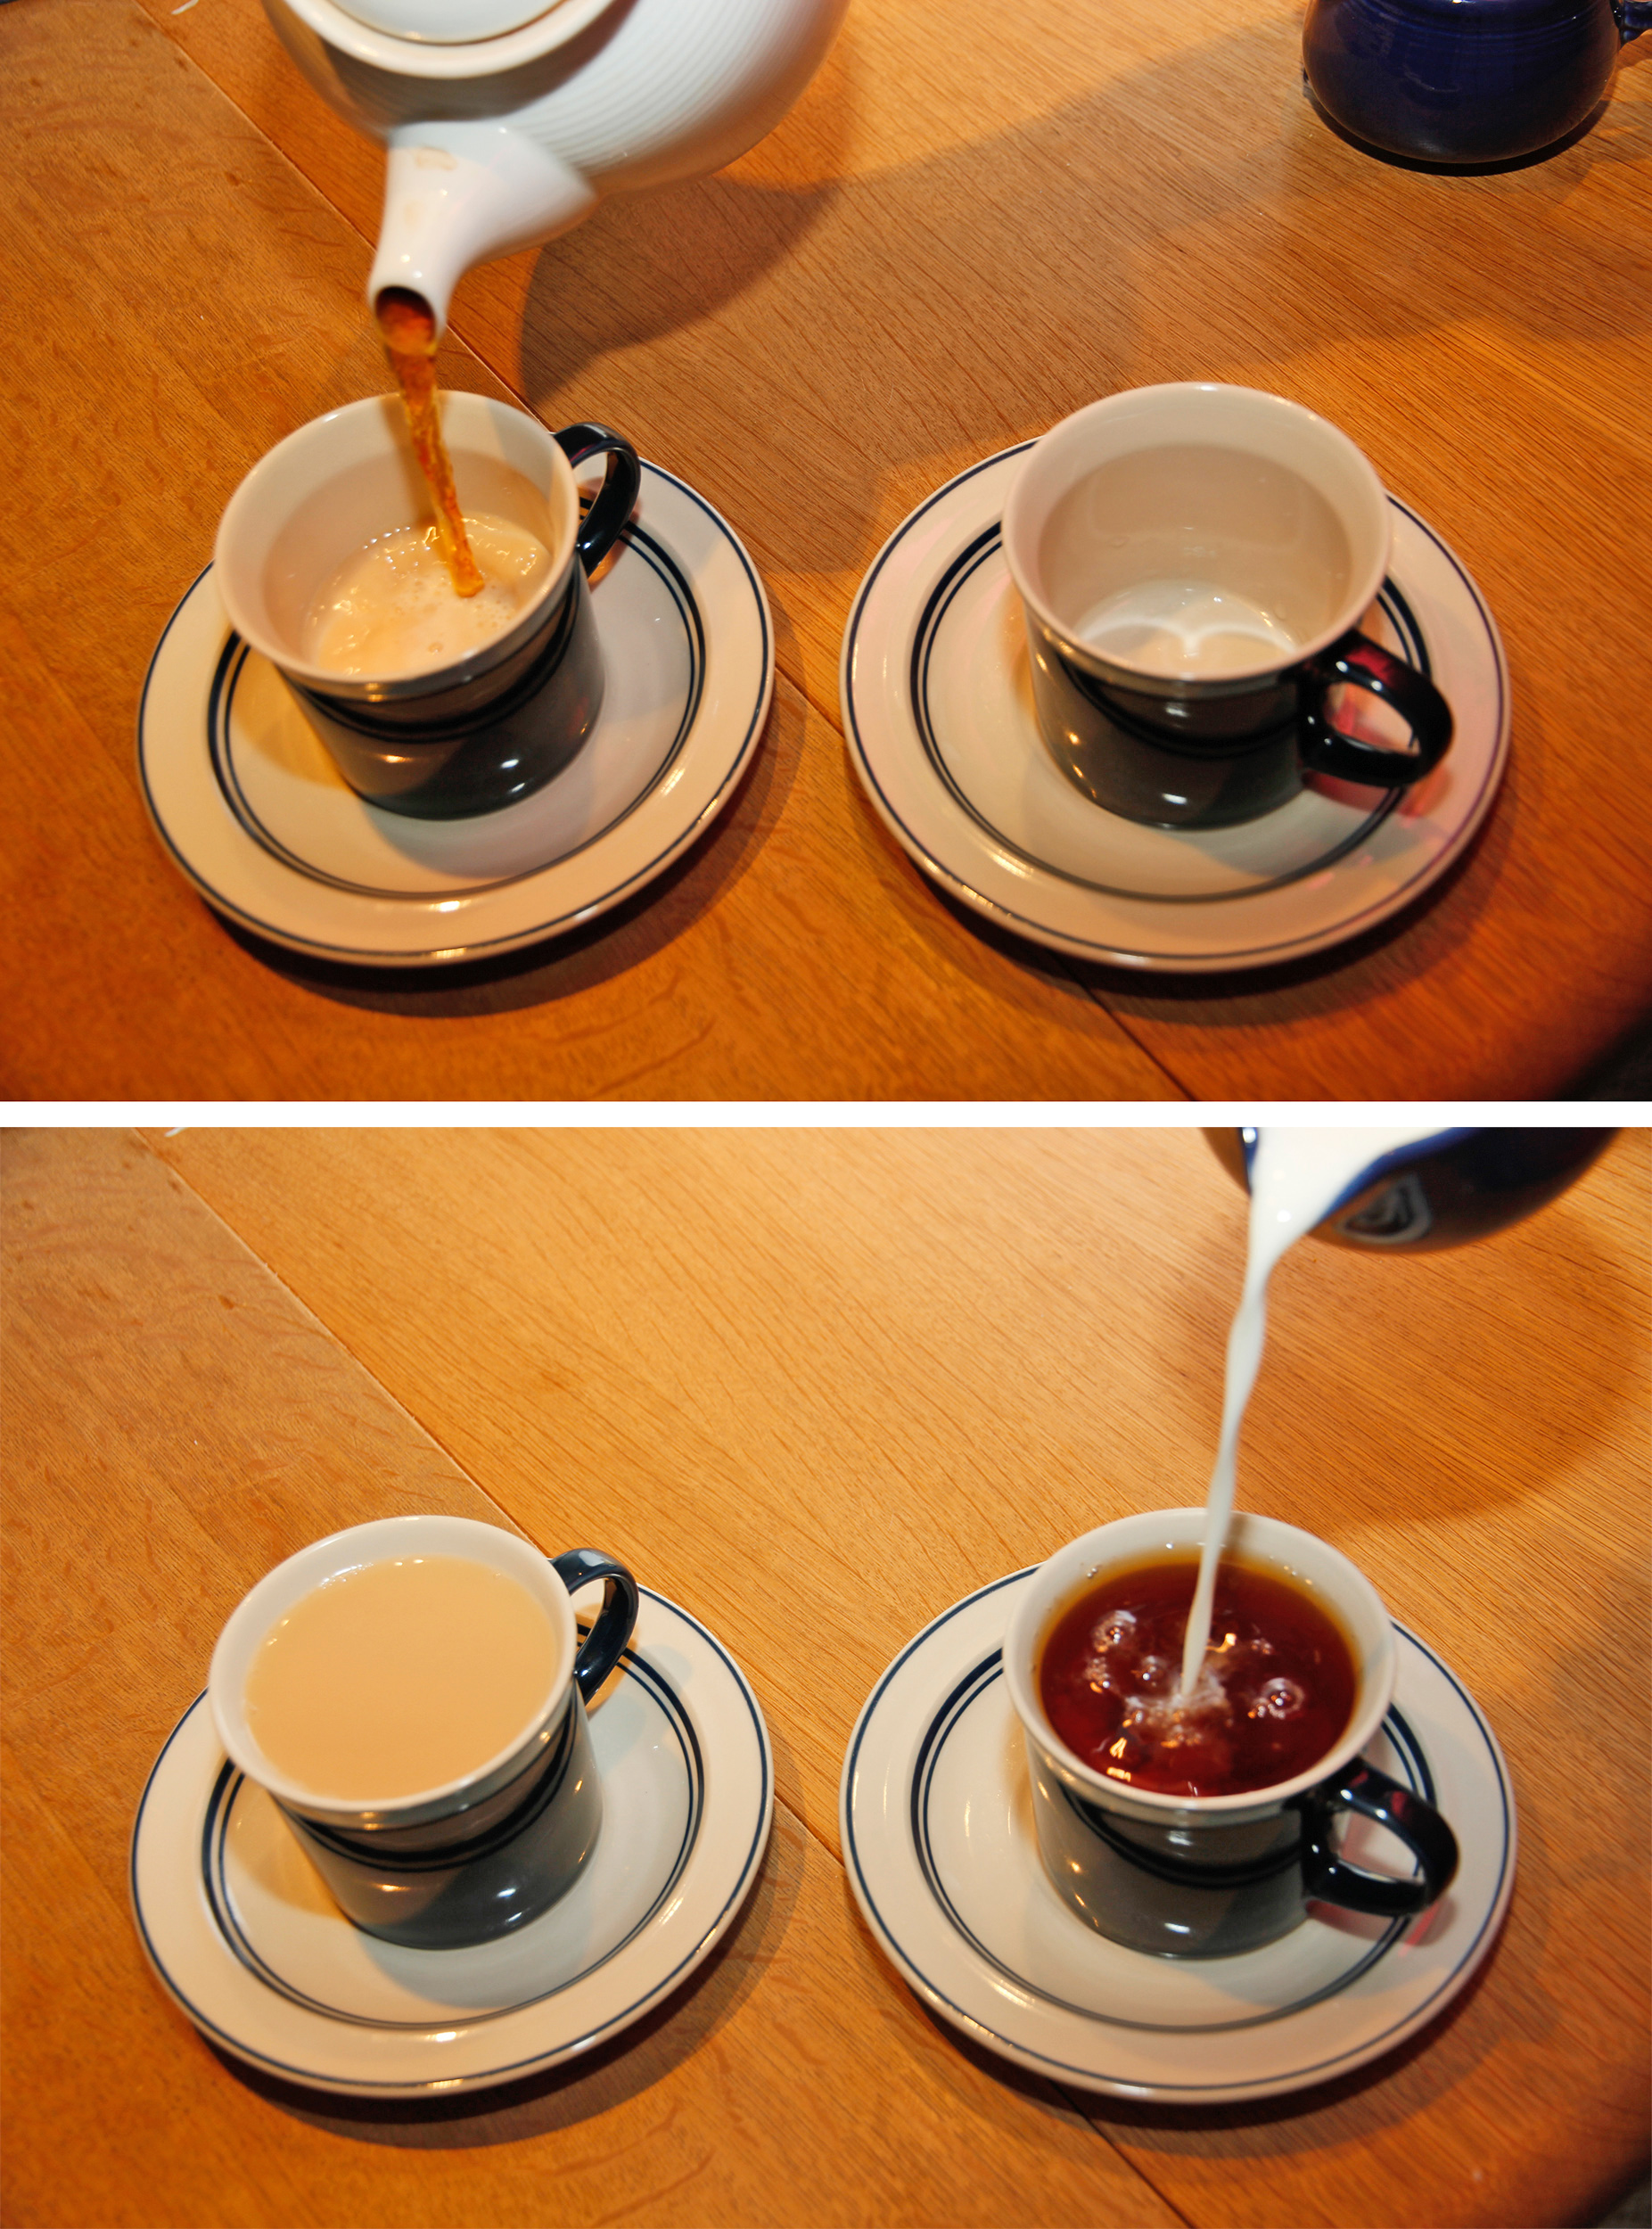
\includegraphics[width=0.4\textwidth]{../Images/TeaFirst_MilkFirst.jpg}\\
  \caption{First milk, then tea (top) - or first tea, then milk (bottom): Could you taste the difference?}\label{fig:ALadyTastingTea}
\end{figure}

\begin{adjustwidth}{2.5em}{2.5em}
    Already, quite soon after he had come to Rothamstead, his presence had transformed one commonplace tea time to an historic event. It happened one afternoon when he drew a cup of tea from the urn and offered it to the lady beside him, Dr. B. Muriel Bristol, an algologist. She declined it, stating that she preferred a cup into which the milk had been poured first. "Nonsense," returned Fisher, smiling, "Surely it makes no difference." But she maintained, with emphasis, that of course it did. From just behind, a voice suggested, "Let's test her." It was William Roach who was not long afterward to marry Miss Bristol. Immediately, they embarked on the preliminaries of the experiment, Roach assisting with the cups and exulting that Miss Bristol divined correctly more than enough of those cups into which tea had been poured first to prove her case.

    Miss Bristol's personal triumph was never recorded, and perhaps Fisher was not satisfied at that moment with the extempore experimental procedure. One can be sure, however, that even as he conceived and carried out the experiment beside the trestle table, and the onlookers, no doubt, took sides as to its outcome, he was thinking through the questions it raised.
\end{adjustwidth}

The real scientific significance of this experiment is in these questions. These are, allowing incidental particulars, the questions one has to consider before designing an experiment. We will look at these questions as pertaining to the "lady tasting tea", but you can imagine how these questions should be adapted to different situations.

\begin{itemize}
  \item \emph{What should be done about chance variations in the temperature, sweetness, and so on?}
    Ideally, one would like to make all cups of tea identical except for the order of pouring milk first or tea first. But it is never possible to control all of the ways in which the cups of tea can differ from each other. If we cannot control these variations, then the best we can do -– we do mean the "best" -– is by randomization.

  \item \emph{How many cups should be used in the test? Should they be paired? In what order should the cups be presented?} The key idea here is that the number and ordering of the cups should allow a subject ample opportunity to prove his or her abilities and keep a fraud from easily succeeding at correctly discriminating the order of pouring in all the cups of tea served.

  \item \emph{What conclusion could be drawn from a perfect score or from one with one or more errors?} If the lady is unable to discriminate between the different orders of pouring, then by guessing alone, it should be highly unlikely for that person to determine correctly which cups are which for all of the cups tested. Similarly, if she indeed possesses some skill at differentiating between the orders of pouring, then it may be unreasonable to require her to make no mistakes so as to distinguish her ability from a pure guesser.

\end{itemize}

An actual scenario described by Fisher and told by many others as the "lady tasting tea" experiment is as follows.

\begin{itemize}
  \item For each cup, we record the order of actual pouring and what the lady says the order is. We can summarize the result by a table like this:

      \begin{tabular}{ r r|c|c|c }
       & \multicolumn{1}{c}{} & \multicolumn{2}{ c }{Order of actual pouring} & \\
       & \multicolumn{1}{c}{} &  \multicolumn{1}{c}{Tea first} & \multicolumn{1}{c}{Milk first} & \\
       \cline{3-4}
       \multirow{2}{*}{Lady says} & Tea first & $a$ & $b$ & $a+b$ \\
       \cline{3-4}
        & Milk first & $c$ & $d$ & $c+d$ \\
       \cline{3-4}
        &  \multicolumn{1}{c}{} & \multicolumn{1}{c}{$a+c$} & \multicolumn{1}{c}{$b+d$} & n \\
      \end{tabular}


      Here $n$ is the total number of cups of tea made. The number of cups where tea is poured
    first is $a + c$ and the lady classifies $a + b$ of them as tea first. Ideally, if she can taste the difference, the counts $b$ and $c$ should be small. On the other hand, if she cannot really tell, we would expect $a$ and $c$ to be about the same.

  \item Suppose now that to test the lady, 8 cups of tea are prepared, 4 tea first, 4 milk first, and she is informed of the design (that there are 4 cups milk first and 4 cups tea first). Suppose also that the cups are presented to her in random order. Her task then is to identify the 4 cups milk first and 4 cups tea first.

    This design fixes the row and column totals in the table above to be 4 each. That is,

    \begin{equation*}
      a + b = a + c = c + d = b + d =4.
    \end{equation*}

    With these constraints, when any one of $a, b, c, d$ is specified, the remaining three are uniquely determined:
    \begin{equation*}
      b =4 - a,\, c =4 - a, \textrm{ and } d = a
    \end{equation*}

    In general, for this design, no matter how many cups ($n$) are served, the row total $a + b$ will equal $a + c$ because the subject knows how many of the cups are "tea first" (or one kind as supposed to the other). So once $a$ is given, the other three counts are specified.

  \item We can test the discriminating skill of the lady, if any, by randomizing the order of the cups served. If we take the position that she has no discriminating skill, then the randomization of the order makes the 4 cups chosen by her as tea first equally likely to be any 4 of the 8 cups served. There are $\left( {\begin{array}{*{20}{c}}
8\\
4
\end{array}} \right) = 70$ (in \emph{Python}, choose \lstinline{scipy.misc.comb(8,4,exact=True)}) possible ways to classify 4 of the 8 cups as "tea first". If the subject has no ability to discriminate between two preparations, then by the randomization, each of these 70 ways is equally likely. Only one of 70 ways leads to a completely correct classification. So someone with no discriminating skill has 1/70 chance of making no errors.

  \item It turns out that, if we assume that she has no discriminating skill, the number of correct classifications of tea first ("a" in the table) has a "hypergeometric" probability distribution (\lstinline{hd=stats.hypergeom(8,4,4)} in \emph{Python}). There are 5 possibilities: 0, 1, 2, 3, 4 for $a$ and the corresponding probabilities (and \emph{Python} commands for computing the probabilities) are tabulated below.

      \begin{tabular}{c|c|c}
        Number of correct calls & \emph{Python} command & Probability \\
        \hline
        0 & hd.pmf(0) & 1/70 \\
        1 & hd.pmf(1) & 16/70 \\
        2 & hd.pmf(2) & 36/70 \\
        3 & hd.pmf(3) & 16/70 \\
        4 & hd.pmf(4) & 1/70
      \end{tabular}


  \item With these probabilities, we can compute the p-value for the test of the hypothesis that the lady cannot tell between the two preparations. Recall that the p-value is the probability of observing a result as extreme or more extreme than the observed result assuming the null hypothesis. If she makes all correct calls,the p-value is 1/70 and if she makes one error (3 correct calls) then the p-value is $1/70 + 16/70 \sim 0.24$.

\end{itemize}
  	
The test described above is known as "Fisher's exact test."


\subsection{McNemar's Test}\index{general}{test!McNemar's}

Although the McNemar test bears a superficial resemblance to a test of categorical association, as might be performed by a 2x2 chi-square test or a 2x2 Fisher exact probability test, it is doing something quite different. The test of association examines the relationship that exists among the cells of the table. The McNemar test examines the difference between the proportions that derive from the marginal sums of the table (see Table \ref{table:frequencyGeneral}): $p_A=(a+b)/N$ and $p_B=(a+c)/N$. The question in the McNemar test is: do these two proportions, $p_A$ and $p_B$, significantly differ? And the answer it receives must take into account the fact that the two proportions are not independent. The correlation of $p_A$ and $p_B$ is occasioned by the fact that both include the quantity a in the upper left cell of the table.

McNemar's test can be used for example in studies in which patients serve as their own control, or in studies with "before and after" design.

\subsubsection{Example}

In the following example, a researcher attempts to determine if a drug has an effect on a particular disease. Counts of individuals are given in the table, with the diagnosis (disease: present or absent) before treatment given in the rows, and the diagnosis after treatment in the columns. The test requires the same subjects to be included in the before-and-after measurements (matched pairs).

\begin{table}
  \centering
  \begin{tabular}{|c|l l l|}
  \hline
  & \emph{After: present} & \emph{After: absent} & \emph{Row total} \\
  \hline
  \emph{Before: present} & 101 & 121 & 222 \\
  \emph{Before: absent} & 59 & 33 & 92 \\
  \emph{Column total} & 160 & 154 & 314 \\
  \hline
  \end{tabular}

  \caption{McNemar's Test: example}\label{table:McNemarExample}
\end{table}


In this example, the null hypothesis of "marginal homogeneity" would mean there was no effect of the treatment. From the above data, the McNemar test statistic with Yates's continuity correction is

\begin{equation}
    \chi^2 = {(|b-c|-correctionFactor)^2 \over b+c}.
\end{equation}

where $\chi^2$ has a chi-squared distribution with 1 degree of freedom. For small number of sample numbers the \emph{correctionFactor} should be 0.5 (\emph{Yates's correction}) or 1.0 (\emph{Edward's correction}). (For $b + c < 25$, the binomial calculation should be performed, and indeed, most software packages simply perform the binomial calculation in all cases, since the result then is an exact test in all cases.) Using Yates's correction, we get

\begin{equation}
    \chi^2 = {(|121 - 59| - 0.5)^2 \over {121 + 59}}
\end{equation}

has the value 21.01, which is extremely unlikely from the distribution implied by the null hypothesis ($p_b = p_c$). Thus the test provides strong evidence to reject the null hypothesis of no treatment effect.

%[xxx Show that McNemar is similar to logistic regression xxx]
% http://stats.stackexchange.com/questions/63257/relationship-between-mcnemars-test-and-conditional-logistic-regression
% in R:
%-----------------------------
%n <- 100
%do.one <- function(n) {
%  id <- rep(1:n, each=2)
%  case <- rep(0:1, times=n)
%  rs <- rbinom(n*2, 1, 0.5)
%  c(
%    'pclogit' = coef(summary(clogit(case ~ rs + strata(id))))[5],
%    'pmctest' = mcnemar.test(table(rs[case == 0], rs[case == 1]))$p.value
%  )
%}
%
%out <- replicate(1000, do.one(n))

\subsection{Cochran's Q Test}\index{general}{test!Cochran's Q}

Cochran's Q test is a hypothesis test where the response variable can take only two possible outcomes (coded as 0 and 1). It is a non-parametric statistical test to verify if k treatments have identical effects. Cochran's Q test should not be confused with \emph{Cochran's C test}, which is a variance outlier test.

\subsubsection{Example}

12 subjects are asked to perform 3 tasks. The outcome of each task is \emph{success} or \emph{failure}. The results are coded $0$ for \emph{failure} and $1$ for \emph{success}. In the example, subject 1 was successful in task 2, but failed tasks 1 and 3 (see Table \ref{table:CochransQ}).

\begin{table}
  \centering
  \begin{tabular}{|r|r r r|}
  \hline
  \emph{Subject}& \emph{Task 1} & \emph{Task 2} & \emph{Task 3} \\
  \hline
  1  & 0 & 1 & 0 \\
  2  & 1 & 1 & 0 \\
  3  & 1 & 1 & 1 \\
  4  & 0 & 0 & 0 \\
  5  & 1 & 0 & 0 \\
  6  & 0 & 1 & 1 \\
  7  & 0 & 0 & 0 \\
  8  & 1 & 1 & 0 \\
  9  & 0 & 1 & 0 \\
  9  & 0 & 1 & 0 \\
  10 & 0 & 1 & 0 \\
  11 & 0 & 1 & 0 \\
  12 & 0 & 1 & 0 \\
  \hline
  \end{tabular}

  \caption{Cochran's Q Test: Success or failure for 12 subjects on 3 tasks.}\label{table:CochransQ}
\end{table}

The null hypothesis for the Cochran's Q test is that there are no differences between the variables. If the calculated probability $p$ is below the selected significance level, the null-hypothesis is rejected, and it can be concluded that the proportions in at least 2 of the variables are significantly different from each other. For our example (Table \ref{table:CochransQ}), the analysis of the data provides $Cochran's Q = 8.6667$ and a significance of $p = 0.013$. In other words, at least one of the three Tasks is easier or harder than the others.

\section{Analysis Programs}

With computers, the computational steps are trivial:

\PyImg "compGroups.py" (p \pageref{py:compGroups}): Analysis of categorical data.
\index{python}{compGroups}

\section{Exercises}

\subsection*{Fisher's Exact Test - The Tea Experiment}

At a party, a lady claimed to be able to tell whether the tea or the milk was added first to a cup. Fisher proposed to give her eight cups, four of each variety, in random order. One could then ask what the probability was for her getting the number she got correct, but just by chance.

The experiment provided the Lady with 8 randomly ordered cups of tea - 4 prepared by first adding milk, 4 prepared by first adding the tea. She was to select the 4 cups prepared by one method. (This offered the Lady the advantage of judging cups by comparison.)

The null hypothesis was that the Lady had no such ability. (In the real, historical experiment, the lady got all eight cups correct.)

\begin{itemize}
  \item Calculate if the claim of the lady is supported if she gets three out of the four pairs correct.\\
  (Correct answer: No. If she gets three correct, that chance that a selection of "three or greater" was random is 0.243. She needs to get all four correct, if we set the rejection threshold at 0.05)

\end{itemize}


\subsection*{Chi2 Contingency Test (1 DOF)}

A test of the effect of a new drug on the heart rate has yielded the following results:

\begin{table}[h]
  \centering
  \begin{tabular}{|c|l l | l|}
  \hline
  & \emph{Heart rate increased} & \emph{Heart rate NOT increased} & \emph{Row total} \\
  \hline
  \emph{Treated} & 36 & 14 & 50 \\
  \emph{Not treated} & 30 & 25 & 55 \\
  \hline
  \emph{Column total} & 66 & 39 & 105 \\
  \hline
  \end{tabular}
\end{table}

\begin{itemize}
  \item     Does the drug affect the heart rate?
    (Correct answer: no)

  \item     What would be the result if the response in one of the not-treated persons would have been different? Perform this test with and without the Yates-correction.
      (Correct anwer:
        without Yates correction: yes, p=0.042\\
        with Yates correction: no, p=0.067)

\end{itemize}

\begin{table}[h]
  \centering
  \begin{tabular}{|c|l l | l|}
  \hline
  & \emph{Heart rate increased} & \emph{Heart rate NOT increased} & \emph{Row total} \\
  \hline
  \emph{Treated} & 36 & 14 & 50 \\
  \emph{Not treated} & 29 & 26 & 55 \\
  \hline
  \emph{Column total} & 65 & 40 & 105 \\
  \hline
  \end{tabular}
\end{table}


\subsection*{One way Chi2-Test ($>1$ DOF)}

The city of Linz wants to know if people want to build a long beach along the Danube. They interview local people, and decide to collect 20 responses from each of the five age groups: ($<15$, 15-30, 30-45, 45-60, $>60$)

The questionnaire states: \emph{"A beachside development will benefit Linz."}

and the possible answers are

\begin{table}[h]
    \centering
    \begin{tabular}{c|c|c|c}
      1 & 2 & 3 & 4 \\
      \hline
      Strongly agree & Agree & Disagree & Strongly Disagree \\
    \end{tabular}
\end{table}

The city council wants to find out if the age of people influenced feelings about the development, particularly of those who felt negatively (i.e. "disagreed" or "strongly disagreed") about the planned development.

\begin{table}[h]
    \centering
    \begin{tabular}{c|c}
      Age group (type) &	Frequency of negative responses (Observed values)\\
      \hline
      $<15$ & 4 \\
      15-30 & 6 \\
      30-45 & 14 \\
      45-60 & 10 \\
      $>60$ & 16
    \end{tabular}
\end{table}

The categories seem to show large differences of opinion between the groups.

\begin{itemize}
  \item     Are these differences significant?
    (Correct answer: yes, p=0.034)

  \item     How many degrees of freedom does the resulting analysis have?
    (Correct answer: 4)

\end{itemize}

\subsection*{McNemar's Test}

In a lawsuit regarding a murder the defense uses a questionnaire to show that the defendant is insane. As a result of the questionnaire, the accused claims "not guilty by reason of insanity".

In reply, the state attorney wants to show that the questionnaire does not work. He hires an experienced neurologist, and presents him with 40 patients, 20 of whom have completed the questionnaire with an "insane" result, and 20 with a "sane" result. When examined by the neurologist, the result is mixed: 19 of the "sane" people are found sane, but 6 of the 20 "insane" people are labelled as sane by the expert.

\begin{table}[h]
  \centering
  \begin{tabular}{|c|l l | l|}
  \hline
  & \emph{sane by expert} & \emph{insane by expert} & \emph{Total} \\
  \hline
  \emph{sane} & 19 & 1 & 20 \\
  \emph{insane} & 6 & 14 & 20 \\
  \hline
  \emph{Total} & 22 & 18 & 40 \\
  \hline
  \end{tabular}
\end{table}


\begin{itemize}
  \item     Is this result significantly different from the questionnaire?
    (Correct answer: no)

  \item     Would the result be significantly different, if the expert had diagnosed all "sane" people correctly?
    (Correct answer: yes)
\end{itemize}
